\documentclass[../../../main.tex]{subfiles}
\begin{document}

\chapter{Testing}
I have not yet created a system where the user can input function so to add layers (this is the only test that I can do at the moment) to the \texttt{PlotPane} I will simply inject the code at the end of the \texttt{PlotPane} constructor to ``add'' layers artificially. Using the table created in the design section I built upon it to create a more suitable tests on the code that I have. I have added tests to test the function in terms of the variable $y$ and to test the Normal Distribution function that I made. The new and updated table is below:

\begin{table}[H]
\begin{tabular}{|c|c|l|l|}
\hline
Test Number        & Function being Tested                                      & \multicolumn{1}{c|}{Sub-Test Number} & Input                          \\ \hline
\multirow{2}{*}{1} & \multirow{2}{*}{Horizontal Lines}                          & a                                    & $4$                            \\ \cline{3-4} 
                   &                                                            & b                                    & $-2$                           \\ \hline
\multirow{2}{*}{2} & \multirow{2}{*}{Linear}                                    & a                                    & $2x-5$                         \\ \cline{3-4} 
                   &                                                            & b                                    & $-0.5x$                        \\ \hline
\multirow{3}{*}{3} & \multirow{3}{*}{Positive Integer Factorised Polynomials}   & a                                    & $x(x-1)$                       \\ \cline{3-4} 
                   &                                                            & b                                    & $x\wedge 2(x\wedge 2+1)$                   \\ \cline{3-4} 
                   &                                                            & c                                    & $-x(3x+1)$                     \\ \hline
\multirow{3}{*}{4} & \multirow{3}{*}{Positive Integer Unfactorised Polynomials} & a                                    & $x\wedge 2+2x+1$                     \\ \cline{3-4} 
                   &                                                            & b                                    & $x\wedge 2-1$                        \\ \cline{3-4} 
                   &                                                            & c                                    & $x\wedge 3+4x\wedge 2+x-6$                 \\ \hline
\multirow{2}{*}{5} & \multirow{2}{*}{Non-Integer Polynomials}                   & a                                    & $x\wedge (1/2)$                      \\ \cline{3-4} 
                   &                                                            & b                                    & $x\wedge (1/3)$                      \\ \hline
\multirow{3}{*}{6} & \multirow{3}{*}{Exponentials}                              & a                                    & $e\wedge x$                          \\ \cline{3-4} 
                   &                                                            & b                                    & $2\wedge x$                          \\ \cline{3-4} 
                   &                                                            & c                                    & $x\wedge x$                          \\ \hline
\multirow{2}{*}{7} & \multirow{2}{*}{Asymptotal}                                & a                                    & $1/(x-1)$                      \\ \cline{3-4} 
                   &                                                            & b                                    & $1/(x-1) + 1/(x+1)$            \\ \hline
\multirow{2}{*}{8} & \multirow{2}{*}{Explicit Functions in terms of $y$}        & a                                    & $y\wedge 2$                          \\ \cline{3-4} 
                   &                                                            & b                                    & $e\wedge y$                          \\ \hline
\multirow{2}{*}{9} & \multirow{2}{*}{Normal Distribution Function}              & a                                    & $\mu = 0$ and $\sigma^ 2 = 1$   \\ \cline{3-4} 
                   &                                                            & b                                    & $\mu = 4$ and $\sigma^ 2 = 0.01$ \\ \hline
10                 & Multiple and Coloured Functions                            & \multicolumn{2}{c|}{N/A}                                              \\ \hline
\end{tabular}
\caption{Prototype 1: Updated Testing Table}
\end{table}

I have laid all of the test evidence into separate sections, with their expected outputs and relevant code. For consistency, I will make every ``a'' sub test black in line colour,  every ``b'' sub test red in line colour and  every ``c'' sub test green in line colour. This also allows me to test another feature of the program. A summary and analysis of the results are recorded in a table at the end of this section.
\newpage
\section{Test 1}
\begin{minted}[
frame=lines,
framesep=2mm,
breaklines
]{java}
ExplicitXFunctionCartesianLayer f = new ExplicitXFunctionCartesianLayer("4");
ExplicitXFunctionCartesianLayer g = new ExplicitXFunctionCartesianLayer("-2");
g.setColor(Color.RED);

this.addLayer(f);
this.addLayer(g);
\end{minted}

\begin{figure}[H]
	\centering
	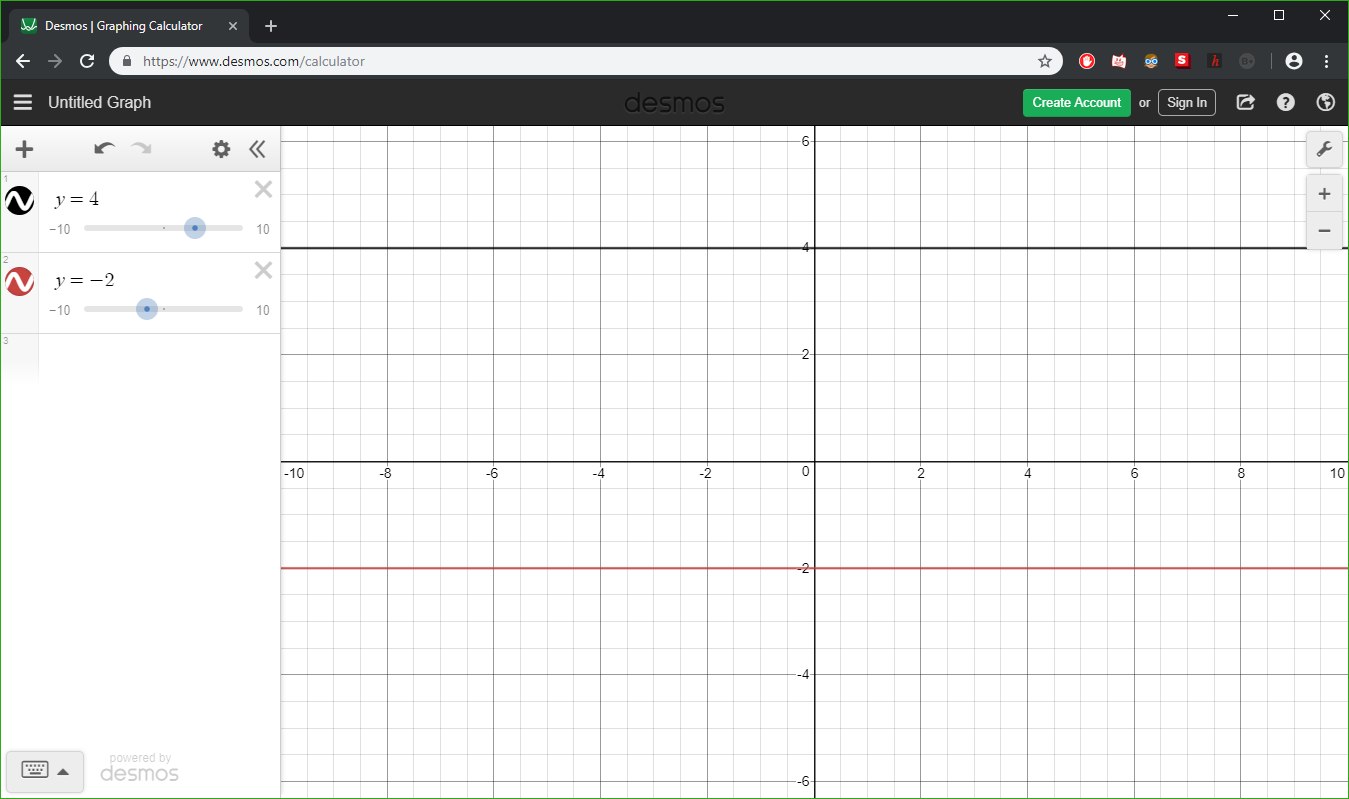
\includegraphics[width=0.6\textwidth]{tests/expected1}
	\caption{Expected Output}
\end{figure}

\begin{figure}[H]
	\centering
	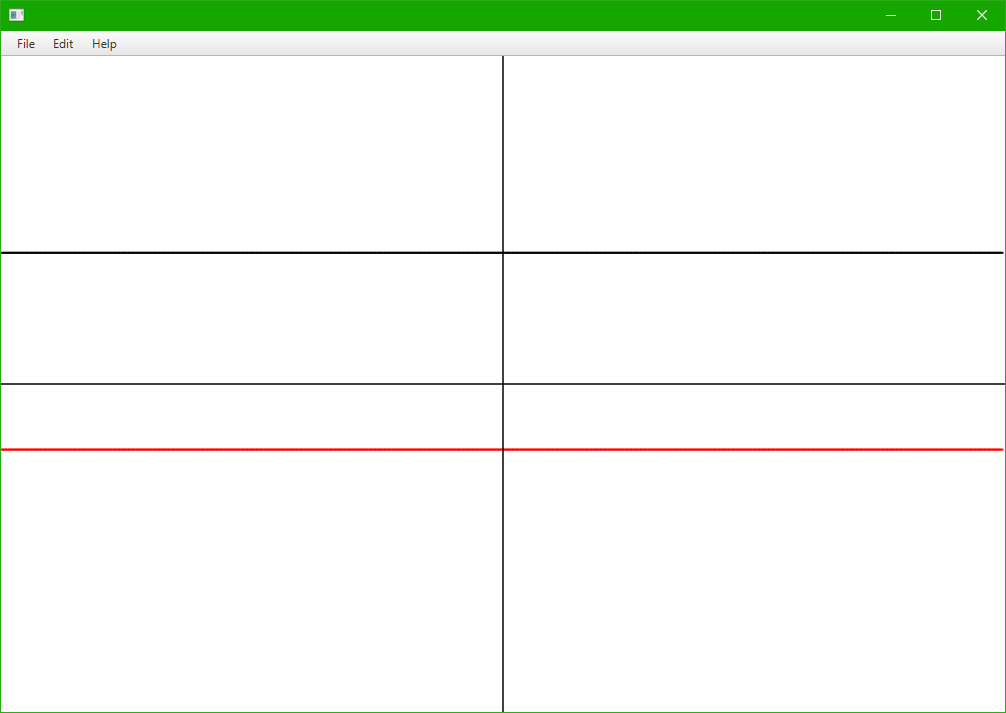
\includegraphics[width=0.6\textwidth]{tests/actual1}
	\caption{Actual Output}
\end{figure}
\newpage

\section{Test 2}
\begin{minted}[
frame=lines,
framesep=2mm,
breaklines
]{java}
ExplicitXFunctionCartesianLayer f = new ExplicitXFunctionCartesianLayer("2x-5");
ExplicitXFunctionCartesianLayer g = new ExplicitXFunctionCartesianLayer("-0.5x");
g.setColor(Color.RED);

this.addLayer(f);
this.addLayer(g);
\end{minted}

\begin{figure}[H]
	\centering
	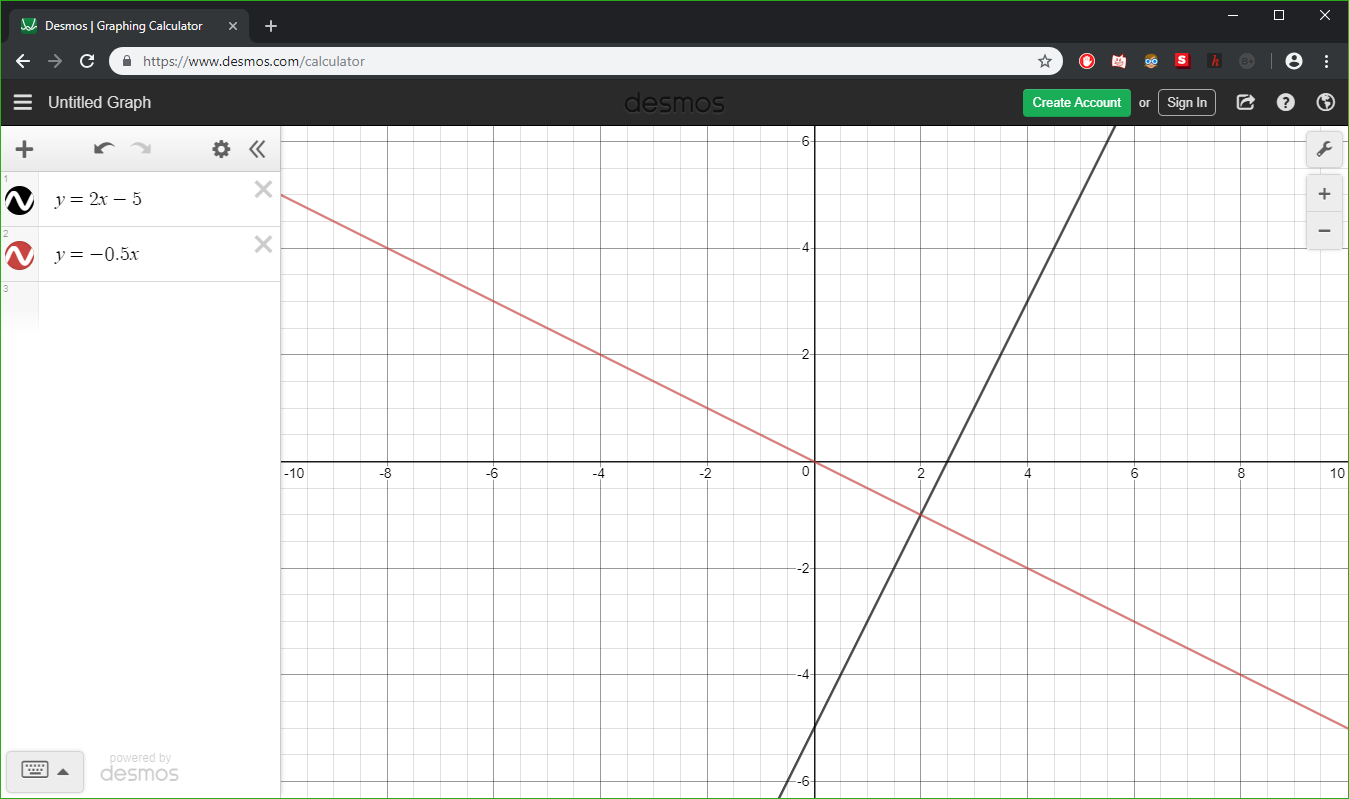
\includegraphics[width=0.6\textwidth]{tests/expected2}
	\caption{Expected Output}
\end{figure}

\begin{figure}[H]
	\centering
	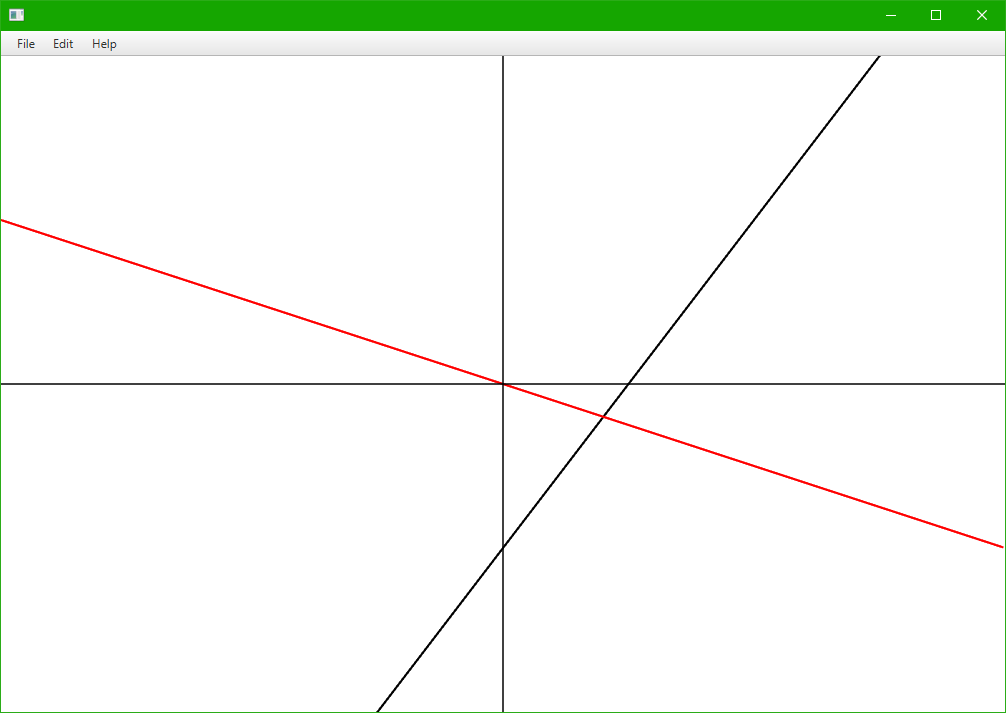
\includegraphics[width=0.6\textwidth]{tests/actual2}
	\caption{Actual Output}
\end{figure}
\newpage

\section{Test 3}
\begin{minted}[
frame=lines,
framesep=2mm,
breaklines
]{java}
ExplicitXFunctionCartesianLayer f = new ExplicitXFunctionCartesianLayer("x(x-1)");
ExplicitXFunctionCartesianLayer g = new ExplicitXFunctionCartesianLayer("x^2(x^2+1)");
ExplicitXFunctionCartesianLayer h = new ExplicitXFunctionCartesianLayer("-x(3x+1)");
g.setColor(Color.RED);
h.setColor(Color.GREEN);

this.addLayer(f);
this.addLayer(g);
this.addLayer(h);
\end{minted}

\begin{figure}[H]
	\centering
	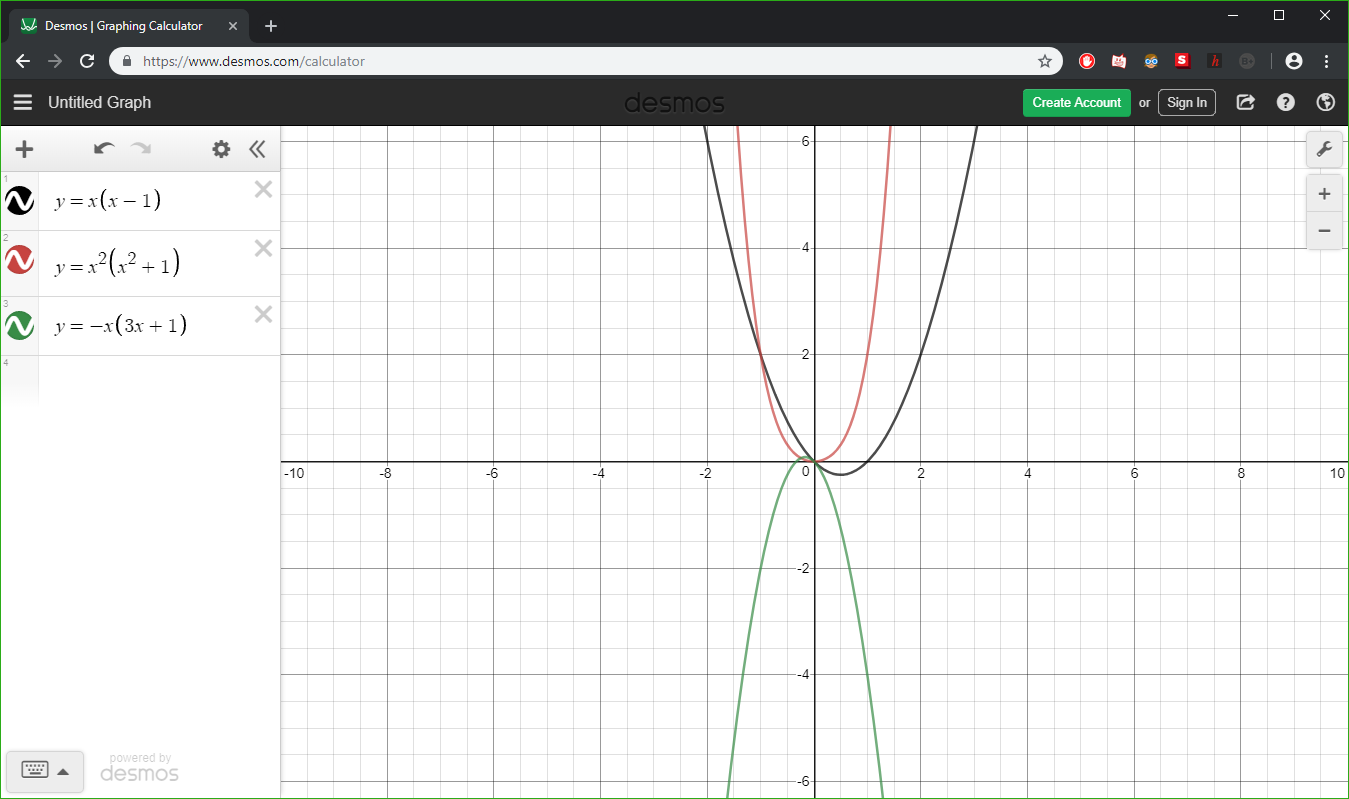
\includegraphics[width=0.6\textwidth]{tests/expected3}
	\caption{Expected Output}
\end{figure}

\begin{figure}[H]
	\centering
	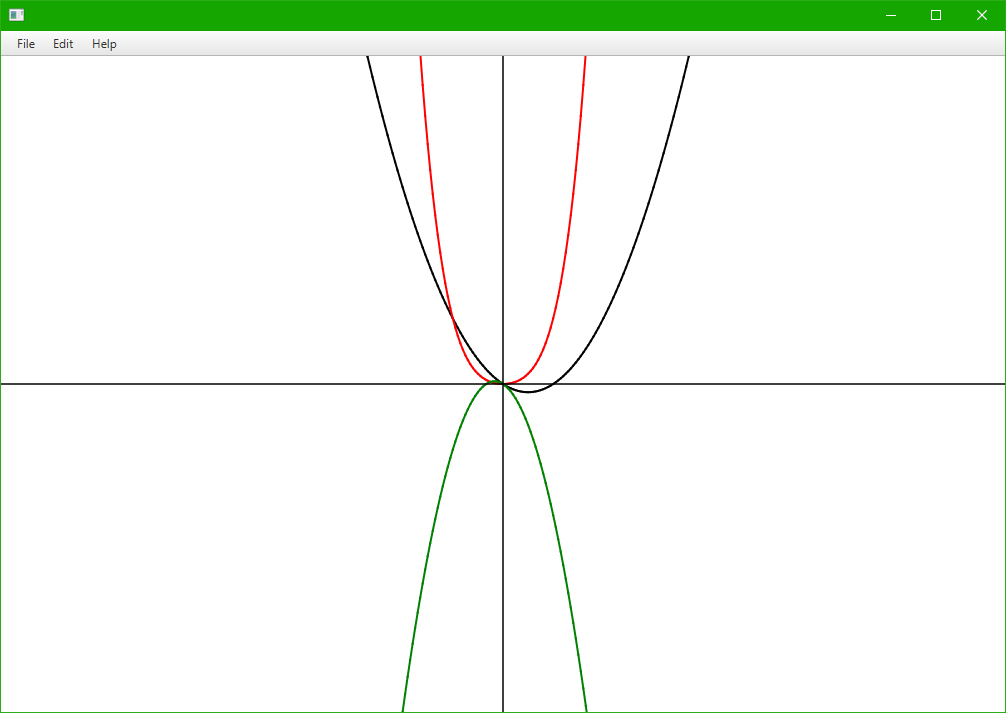
\includegraphics[width=0.6\textwidth]{tests/actual3}
	\caption{Actual Output}
\end{figure}
\newpage

\section{Test 4}
\begin{minted}[
frame=lines,
framesep=2mm,
breaklines
]{java}
ExplicitXFunctionCartesianLayer f = new ExplicitXFunctionCartesianLayer("x^2+2x+1");
ExplicitXFunctionCartesianLayer g = new ExplicitXFunctionCartesianLayer("x^2-1");
ExplicitXFunctionCartesianLayer h = new ExplicitXFunctionCartesianLayer("x^3+4x^2+x-6");
g.setColor(Color.RED);
h.setColor(Color.GREEN);

this.addLayer(f);
this.addLayer(g);
this.addLayer(h);
\end{minted}

\begin{figure}[H]
	\centering
	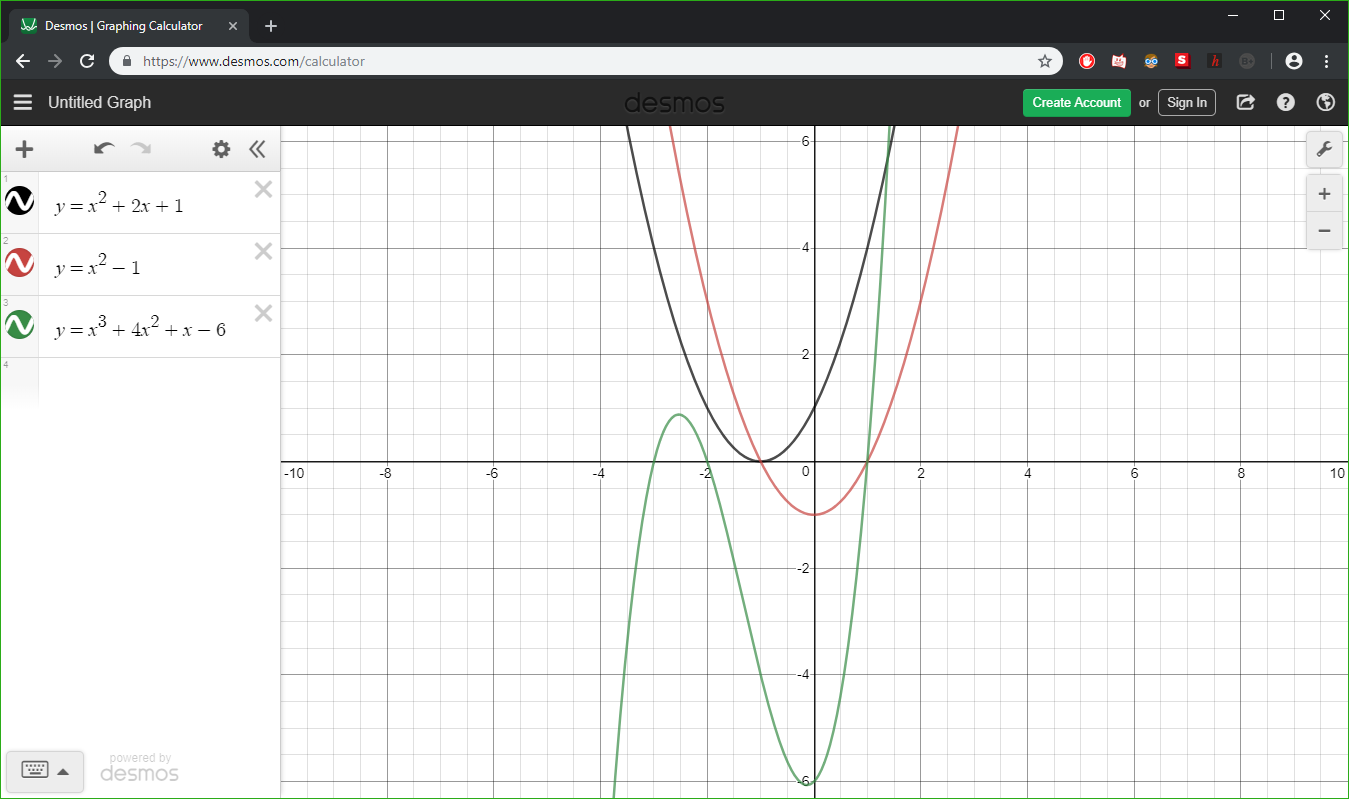
\includegraphics[width=0.6\textwidth]{tests/expected4}
	\caption{Expected Output}
\end{figure}

\begin{figure}[H]
	\centering
	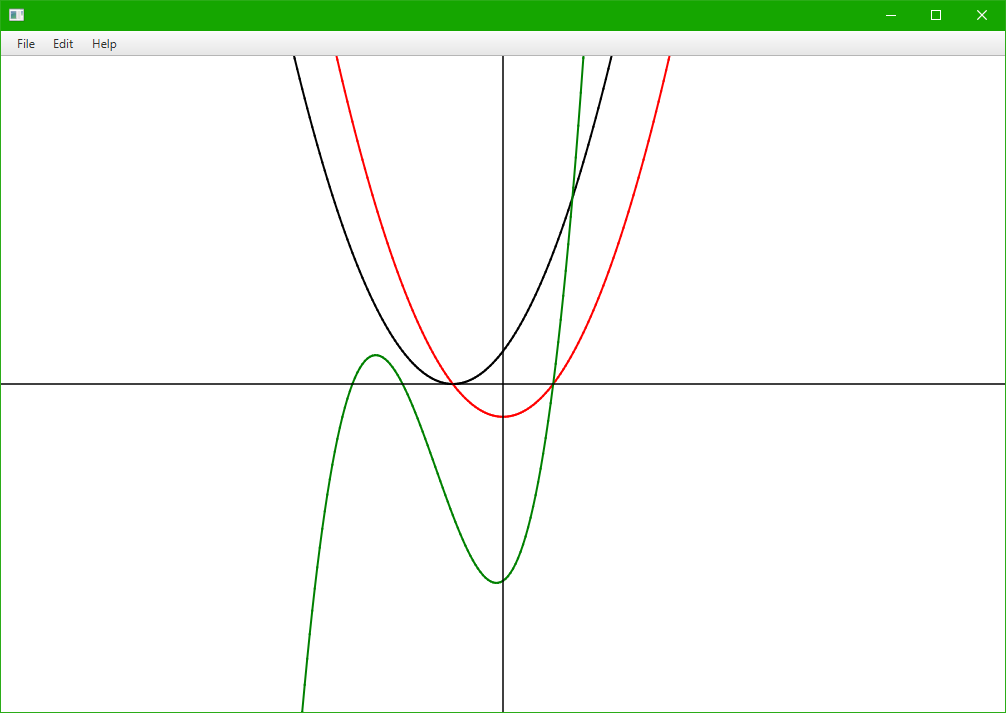
\includegraphics[width=0.6\textwidth]{tests/actual4}
	\caption{Actual Output}
\end{figure}
\newpage

\section{Test 5}
\begin{minted}[
frame=lines,
framesep=2mm,
breaklines
]{java}
ExplicitXFunctionCartesianLayer f = new ExplicitXFunctionCartesianLayer("x^(1/2)");
ExplicitXFunctionCartesianLayer g = new ExplicitXFunctionCartesianLayer("x^(1/3)");
g.setColor(Color.RED);

this.addLayer(f);
this.addLayer(g);
\end{minted}

\begin{figure}[H]
	\centering
	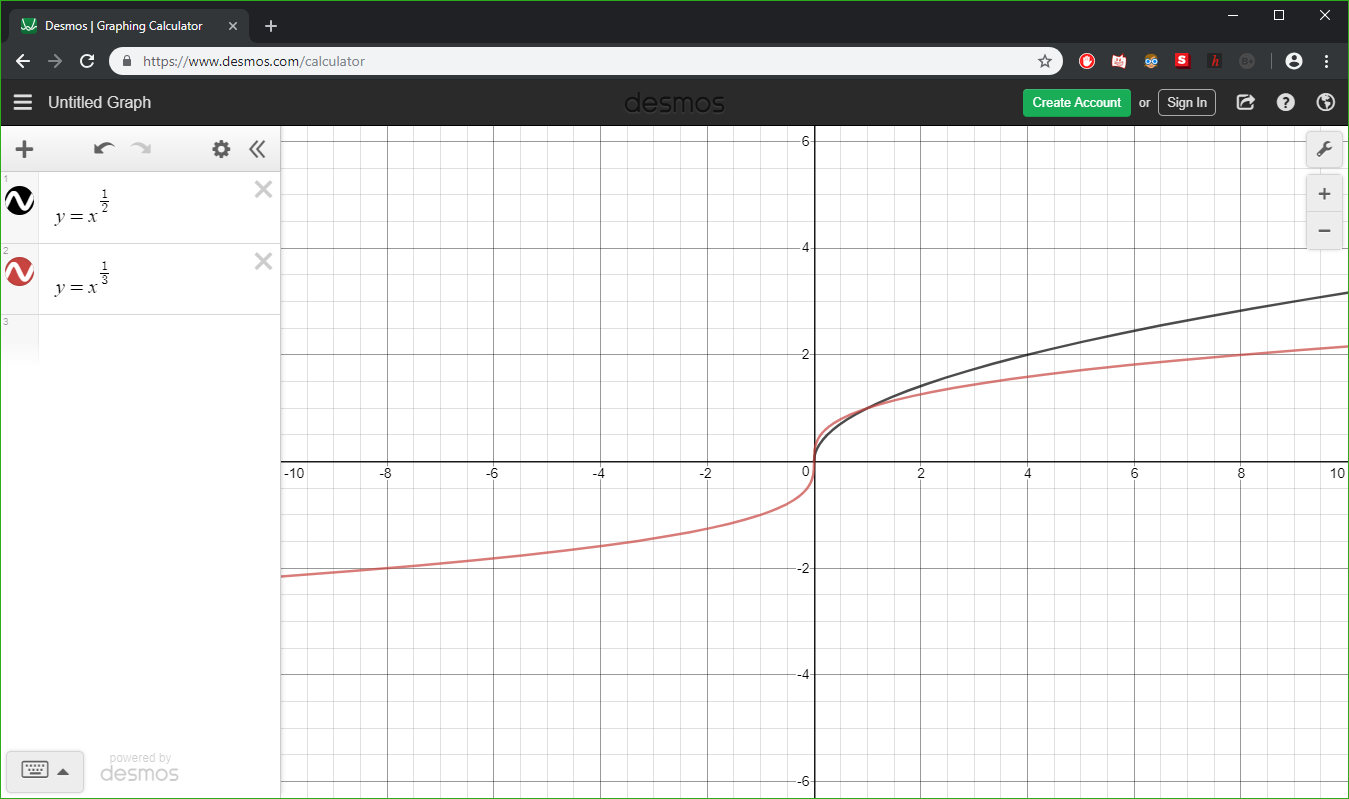
\includegraphics[width=0.6\textwidth]{tests/expected5}
	\caption{Expected Output}
\end{figure}

\begin{figure}[H]
	\centering
	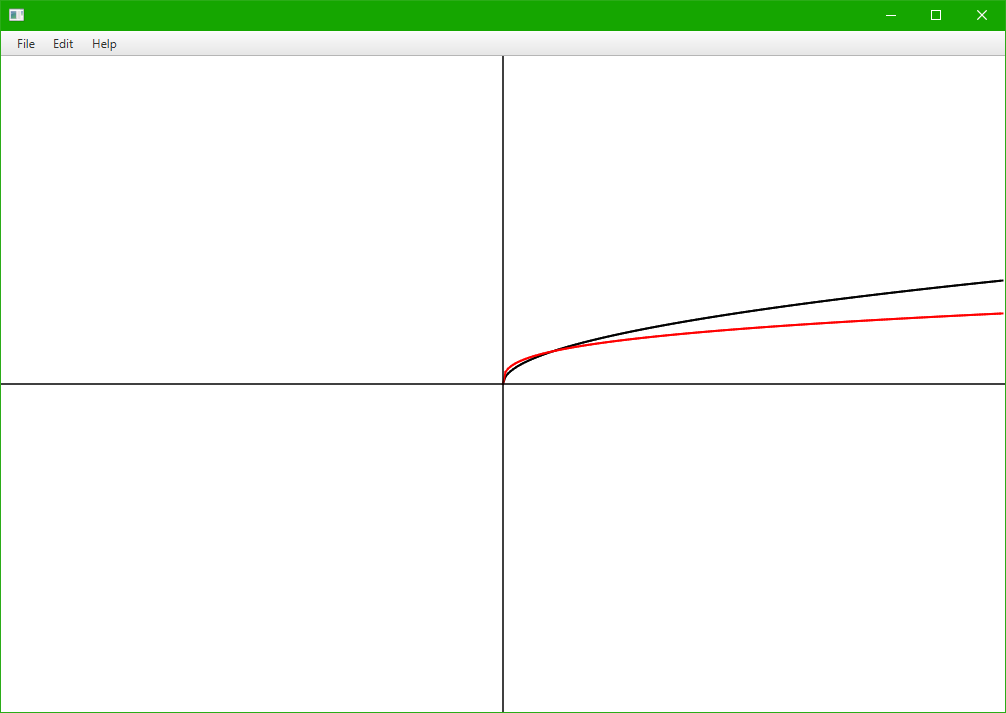
\includegraphics[width=0.6\textwidth]{tests/actual5}
	\caption{Actual Output}
\end{figure}
\newpage

\section{Test 6}
\begin{minted}[
frame=lines,
framesep=2mm,
breaklines
]{java}
ExplicitXFunctionCartesianLayer f = new ExplicitXFunctionCartesianLayer("e^x");
ExplicitXFunctionCartesianLayer g = new ExplicitXFunctionCartesianLayer("2^x");
ExplicitXFunctionCartesianLayer h = new ExplicitXFunctionCartesianLayer("x^x");
g.setColor(Color.RED);
h.setColor(Color.GREEN);

this.addLayer(f);
this.addLayer(g);
this.addLayer(h);
\end{minted}

\begin{figure}[H]
	\centering
	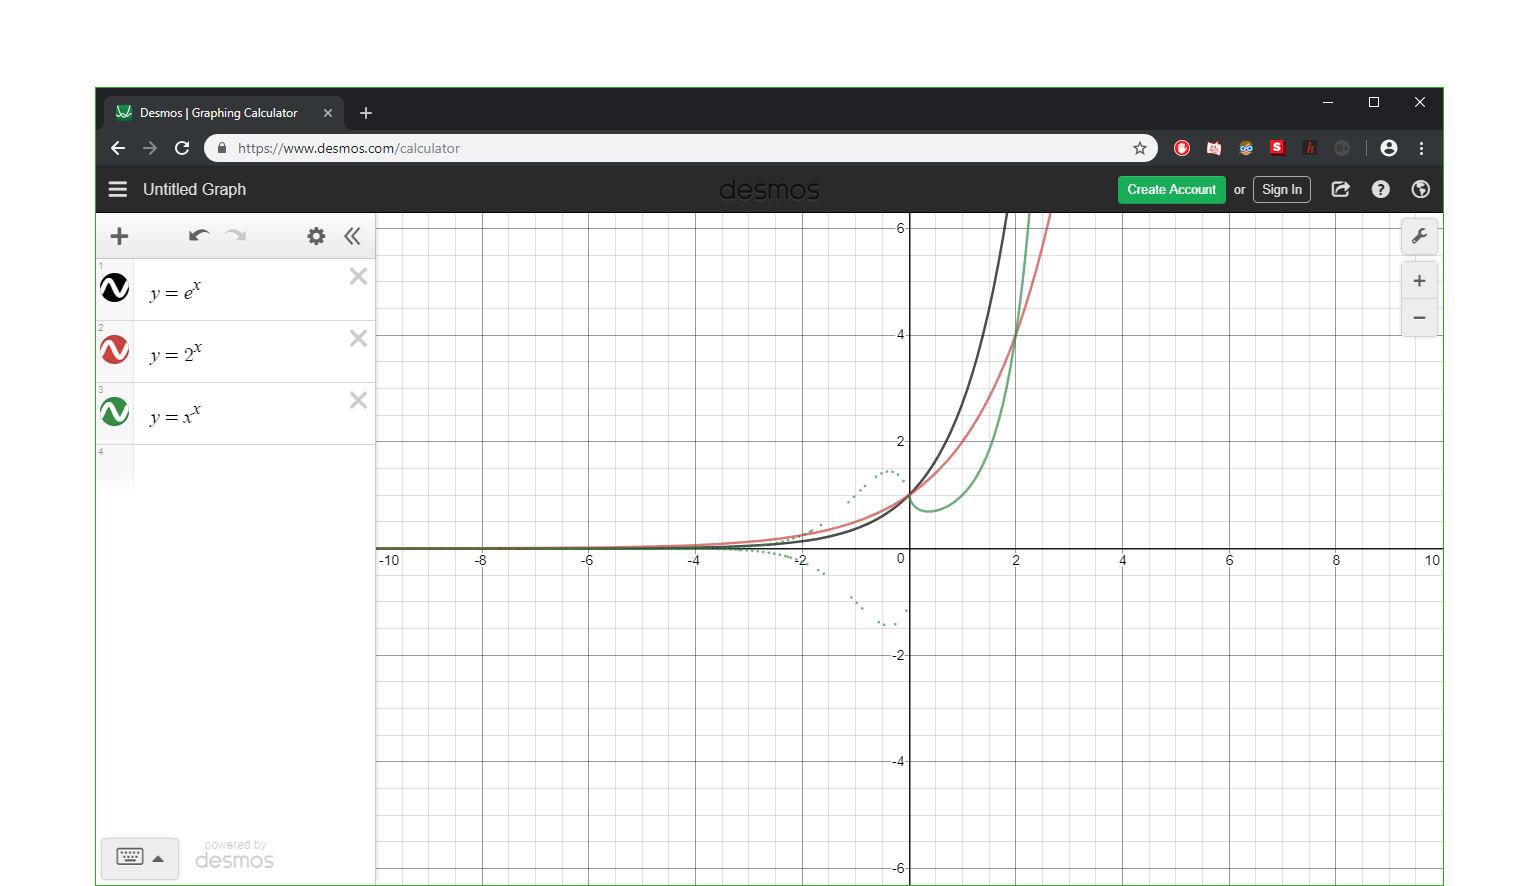
\includegraphics[width=0.6\textwidth]{tests/expected6}
	\caption{Expected Output}
\end{figure}

\begin{figure}[H]
	\centering
	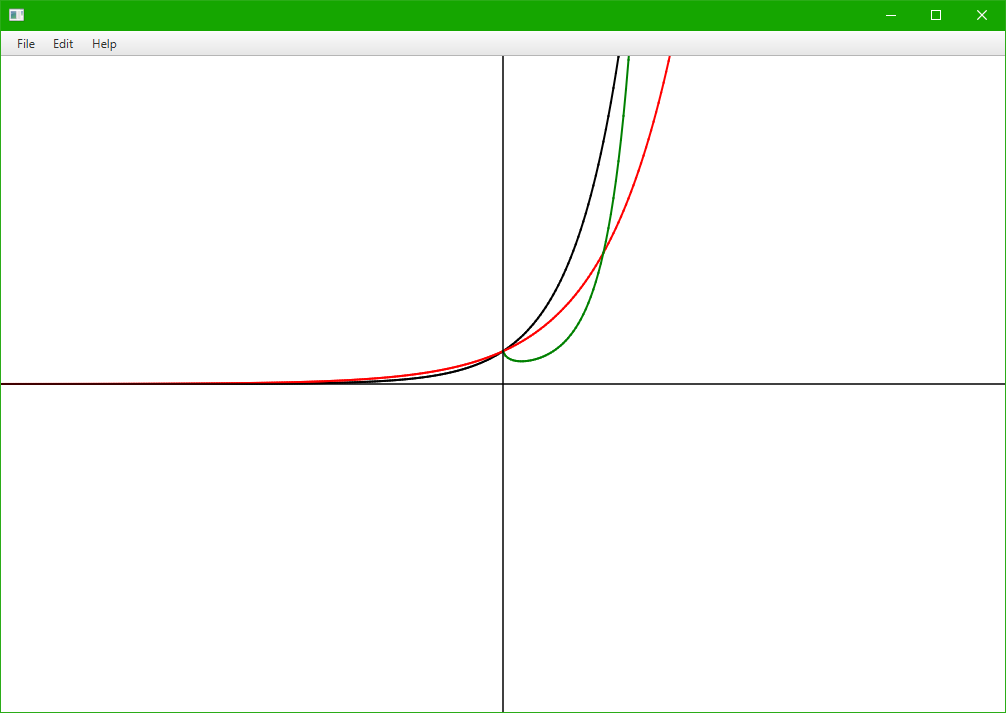
\includegraphics[width=0.6\textwidth]{tests/actual6}
	\caption{Actual Output}
\end{figure}
\newpage

\section{Test 7}
\begin{minted}[
frame=lines,
framesep=2mm,
breaklines
]{java}
ExplicitXFunctionCartesianLayer f = new ExplicitXFunctionCartesianLayer("1/(x-1)");
ExplicitXFunctionCartesianLayer g = new ExplicitXFunctionCartesianLayer("1/(x-1) + 1/(x+1)");
g.setColor(Color.RED);

this.addLayer(f);
this.addLayer(g);
\end{minted}

\begin{figure}[H]
	\centering
	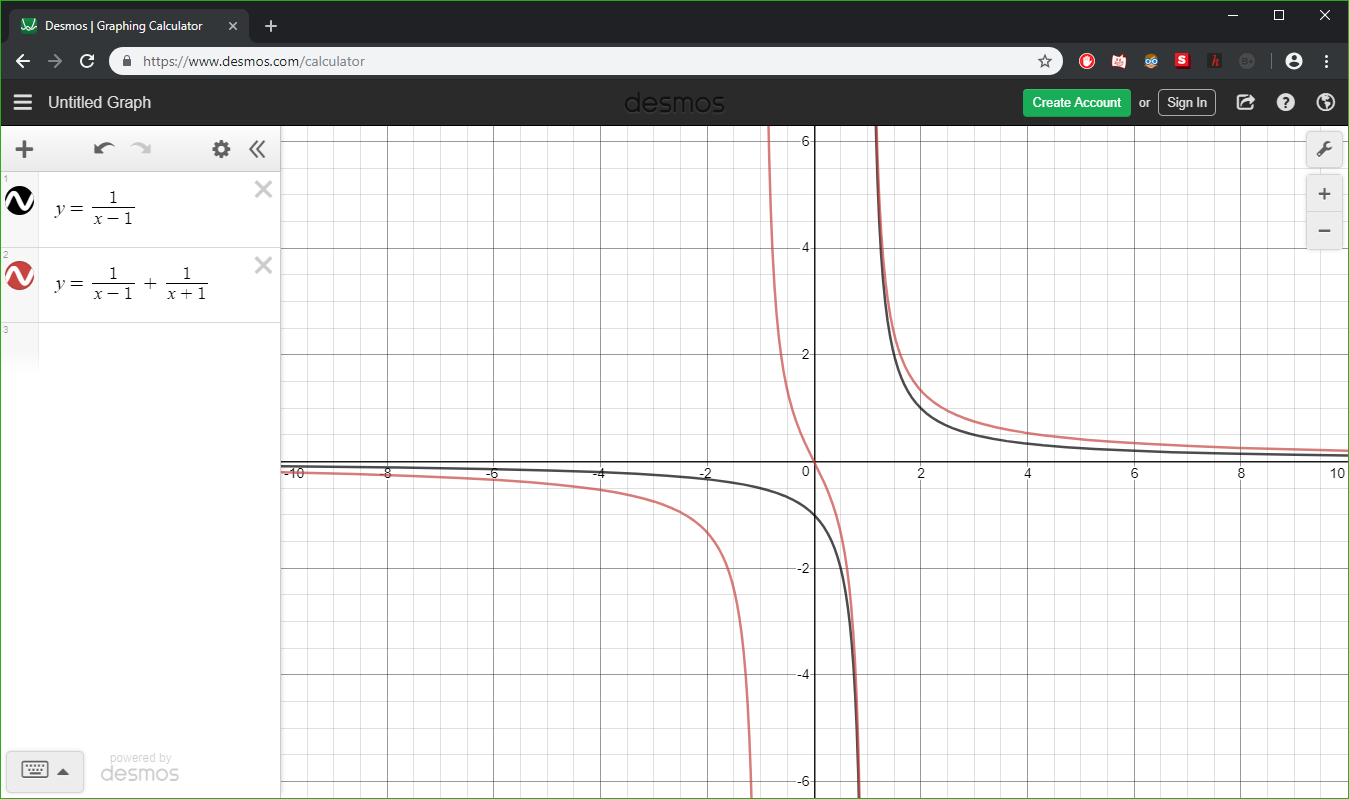
\includegraphics[width=0.6\textwidth]{tests/expected7}
	\caption{Expected Output}
\end{figure}

\begin{figure}[H]
	\centering
	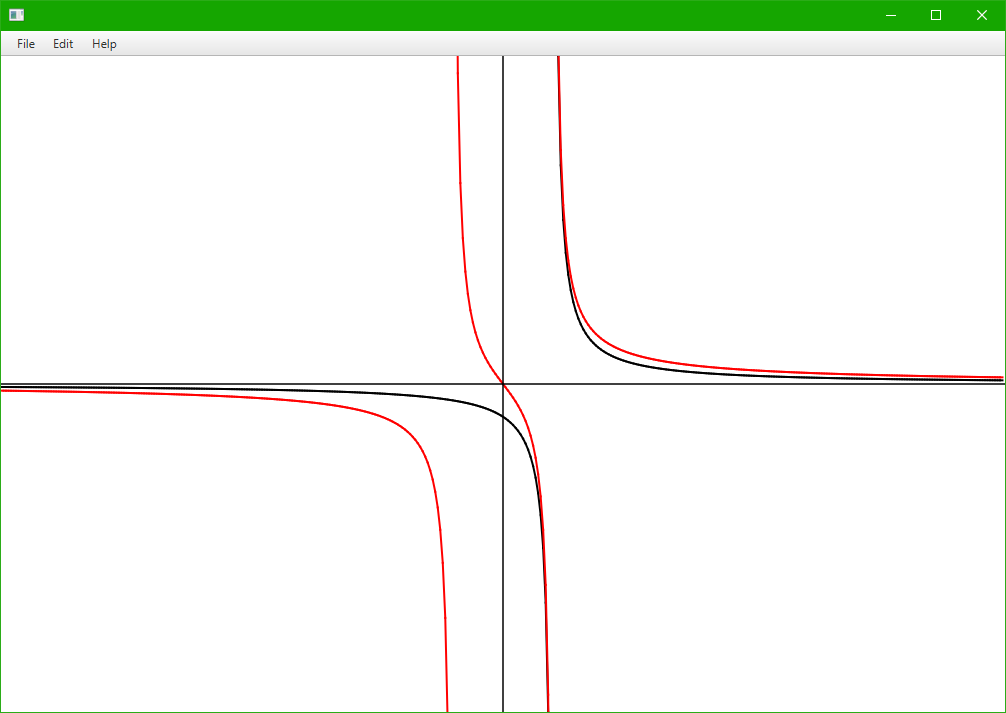
\includegraphics[width=0.6\textwidth]{tests/actual7}
	\caption{Actual Output}
\end{figure}
\newpage

\section{Test 8}
\begin{minted}[
frame=lines,
framesep=2mm,
breaklines
]{java}
ExplicitYFunctionCartesianLayer f = new ExplicitYFunctionCartesianLayer("y^2");
ExplicitYFunctionCartesianLayer g = new ExplicitYFunctionCartesianLayer("e^y");
g.setColor(Color.RED);

this.addLayer(f);
this.addLayer(g);
\end{minted}

\begin{figure}[H]
	\centering
	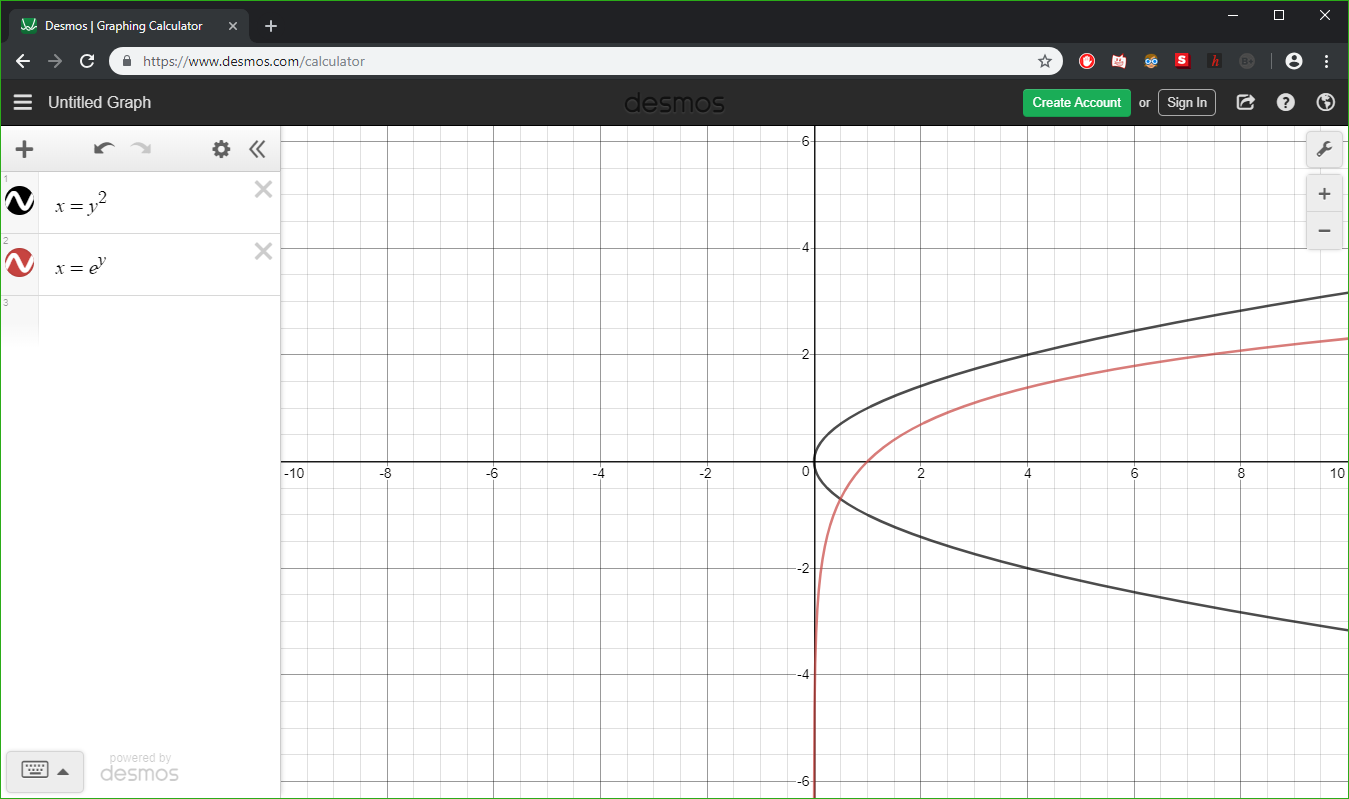
\includegraphics[width=0.6\textwidth]{tests/expected8}
	\caption{Expected Output}
\end{figure}

\begin{figure}[H]
	\centering
	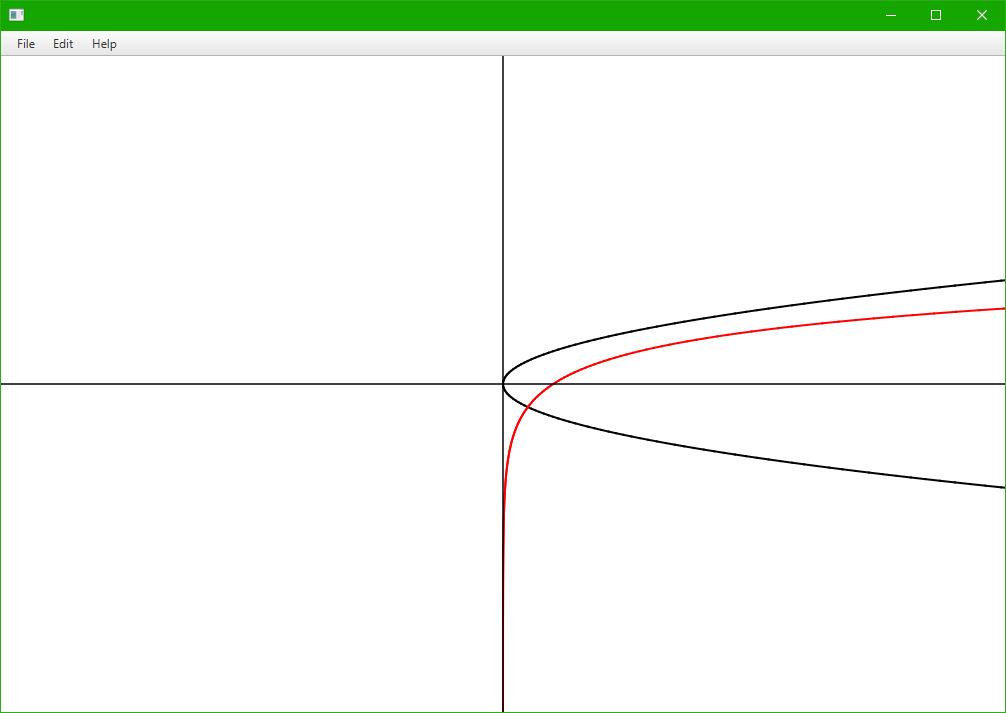
\includegraphics[width=0.6\textwidth]{tests/actual8}
	\caption{Actual Output}
\end{figure}
\newpage

\section{Test 9}
\begin{minted}[
frame=lines,
framesep=2mm,
breaklines
]{java}
ExplicitXFunctionCartesianLayer f = new ExplicitXFunctionCartesianLayer(new NormalDistribution(0, 1));
ExplicitXFunctionCartesianLayer g = new ExplicitXFunctionCartesianLayer(new NormalDistribution(4, 0.01));
g.setColor(Color.RED);

this.addLayer(f);
this.addLayer(g);
\end{minted}

\begin{figure}[H]
	\centering
	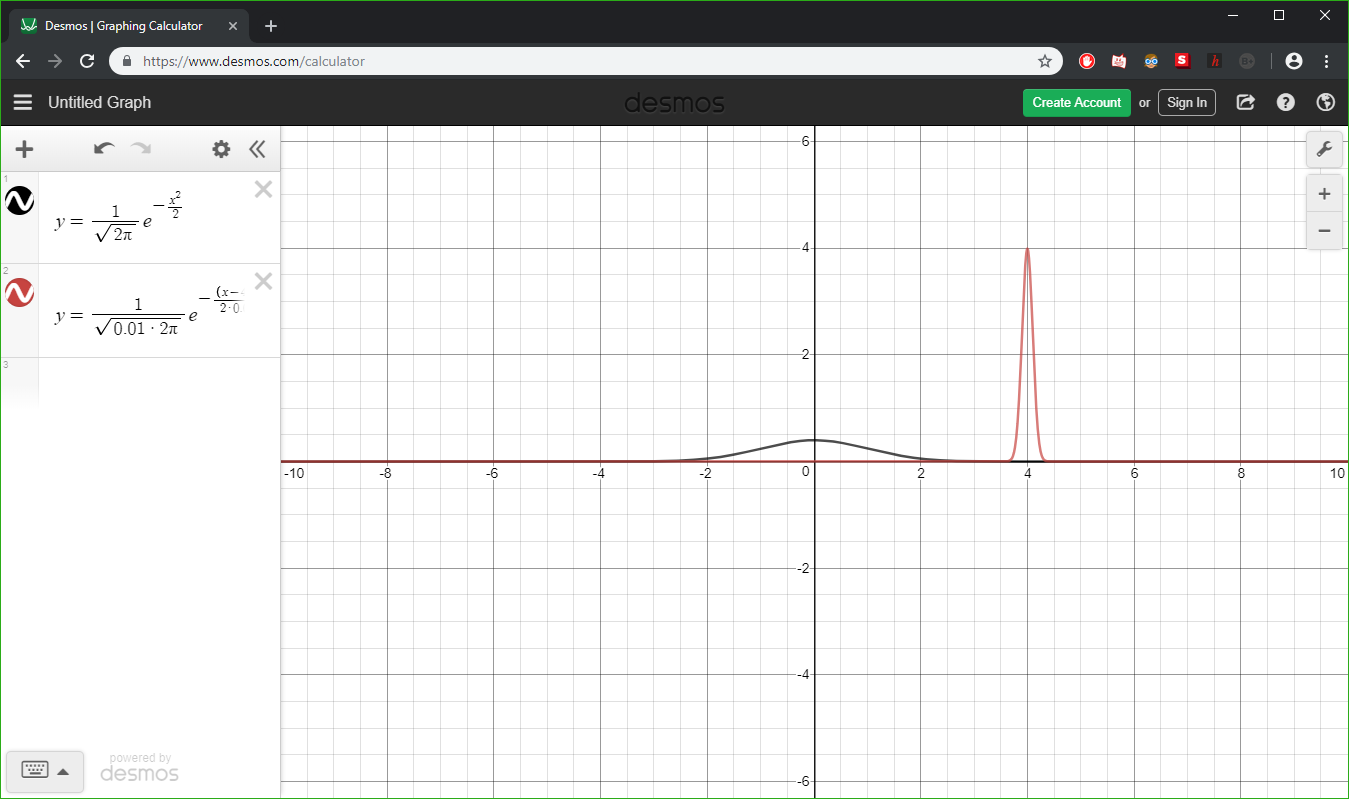
\includegraphics[width=0.6\textwidth]{tests/expected9}
	\caption{Expected Output}
\end{figure}

\begin{figure}[H]
	\centering
	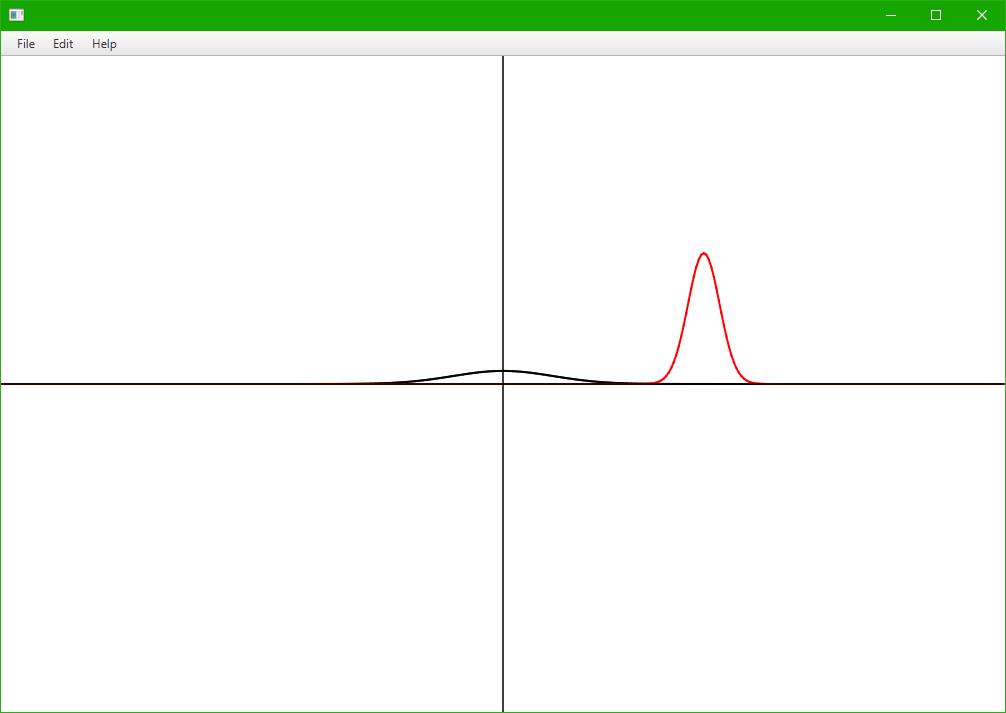
\includegraphics[width=0.6\textwidth]{tests/actual9}
	\caption{Actual Output}
\end{figure}
\newpage
\section{Conclusion}

\begin{table}[H]
\centering
\begin{tabular}{|C{0.08\textwidth}|C{0.15\textwidth}|C{0.1\textwidth}|C{0.55\textwidth}|}
\hline
Test Number & Function being Tested                     & Pass/Fail & Analysis                                                                                                                                                                                                                                                                                                                                                                                                                                                                                                                                                                                                                                                                                                                                                                                           \\ \hline
1           & Horizontal Lines                          & {\Large \cmark}    & The output was exactly what was expected.                                                                                                                                                                                                                                                                                                                                                                                                                                                                                                                                                                                                                                                                                                                                                          \\ \hline
2           & Linear                                    & {\Large \cmark}    & The output was exactly what was expected.                                                                                                                                                                                                                                                                                                                                                                                                                                                                                                                                                                                                                                                                                                                                                          \\ \hline
3           & Positive Integer Factorised Polynomials   & {\Large \cmark}    & The output was exactly what was expected.                                                                                                                                                                                                                                                                                                                                                                                                                                                                                                                                                                                                                                                                                                                                                          \\ \hline
4           & Positive Integer Unfactorised Polynomials & {\Large \cmark}    & The output was exactly what was expected.                                                                                                                                                                                                                                                                                                                                                                                                                                                                                                                                                                                                                                                                                                                                                          \\ \hline
5           & Non-Integer Polynomials                   & {\Large \xmark}    & Test part b partially failed since for $x<0$ there was nothing drawn. This is due to the function \texttt{Math.pow()} returning \texttt{NaN}, Not a Number, when given a negative base and a non-integer index\cite{powJava}. This is a limitation of the language I am using and I cannot do anything about it. \\ \hline
6           & Exponentials                              & {\Large \xmark}    & Test part c partially failed. Looking closely at the two images you can see that there were individual points for $x<0$ in the expected result where the function existed. However in the actual result, there was nothing drawn. This seems to be due to there only being one value in the local range for which the function is valid. Since our program works by connecting many points together with a straight line it makes sense that it doesn't work for single points. While this is a loss in accuracy, one of the targets for this project was for a responsive application and if we used a pixel by pixel drawing algorithm it would be too slow. So this is not worth attempting to fix since it would go against one of the targets for this projects. \\ \hline
7           & Asymptotal                                & {\Large \cmark}    & The output was exactly what was expected.                                                                                                                                                                                                                                                                                                                                                                                                                                                                                                                                                                                                                                                                                                                                                          \\ \hline
8           & Explicit Functions in terms of $y$        & {\Large \cmark}    & The output was exactly what was expected.                                                                                                                                                                                                                                                                                                                                                                                                                                                                                                                                                                                                                                                                                                                                                          \\ \hline
9           & Normal Distribution Function              & {\Large \cmark}    & The output was exactly what was expected.                                                                                                                                                                                                                                                                                                                                                                                                                                                                                                                                                                                                                                                                                                                                                          \\ \hline
10          & Multiple and Coloured Functions            & {\Large \cmark}    & The multiple functions and different colours for all the separate functions worked perfectly for all the tests.                                                                                                                                                                                                                                                                                                                                                                                                                                                                                                                                                                                                                                                                             \\ \hline
\end{tabular}
\caption{Conclusion and Analysis of the Prototype 1 Tests}
\end{table}
\newpage
\end{document}